
    {
        \newcommand{\tempwidth}[0]{0.8\linewidth}
        \begin{figure}
             \centering
             \begin{subfigure}{\textwidth}
                 \centering
                 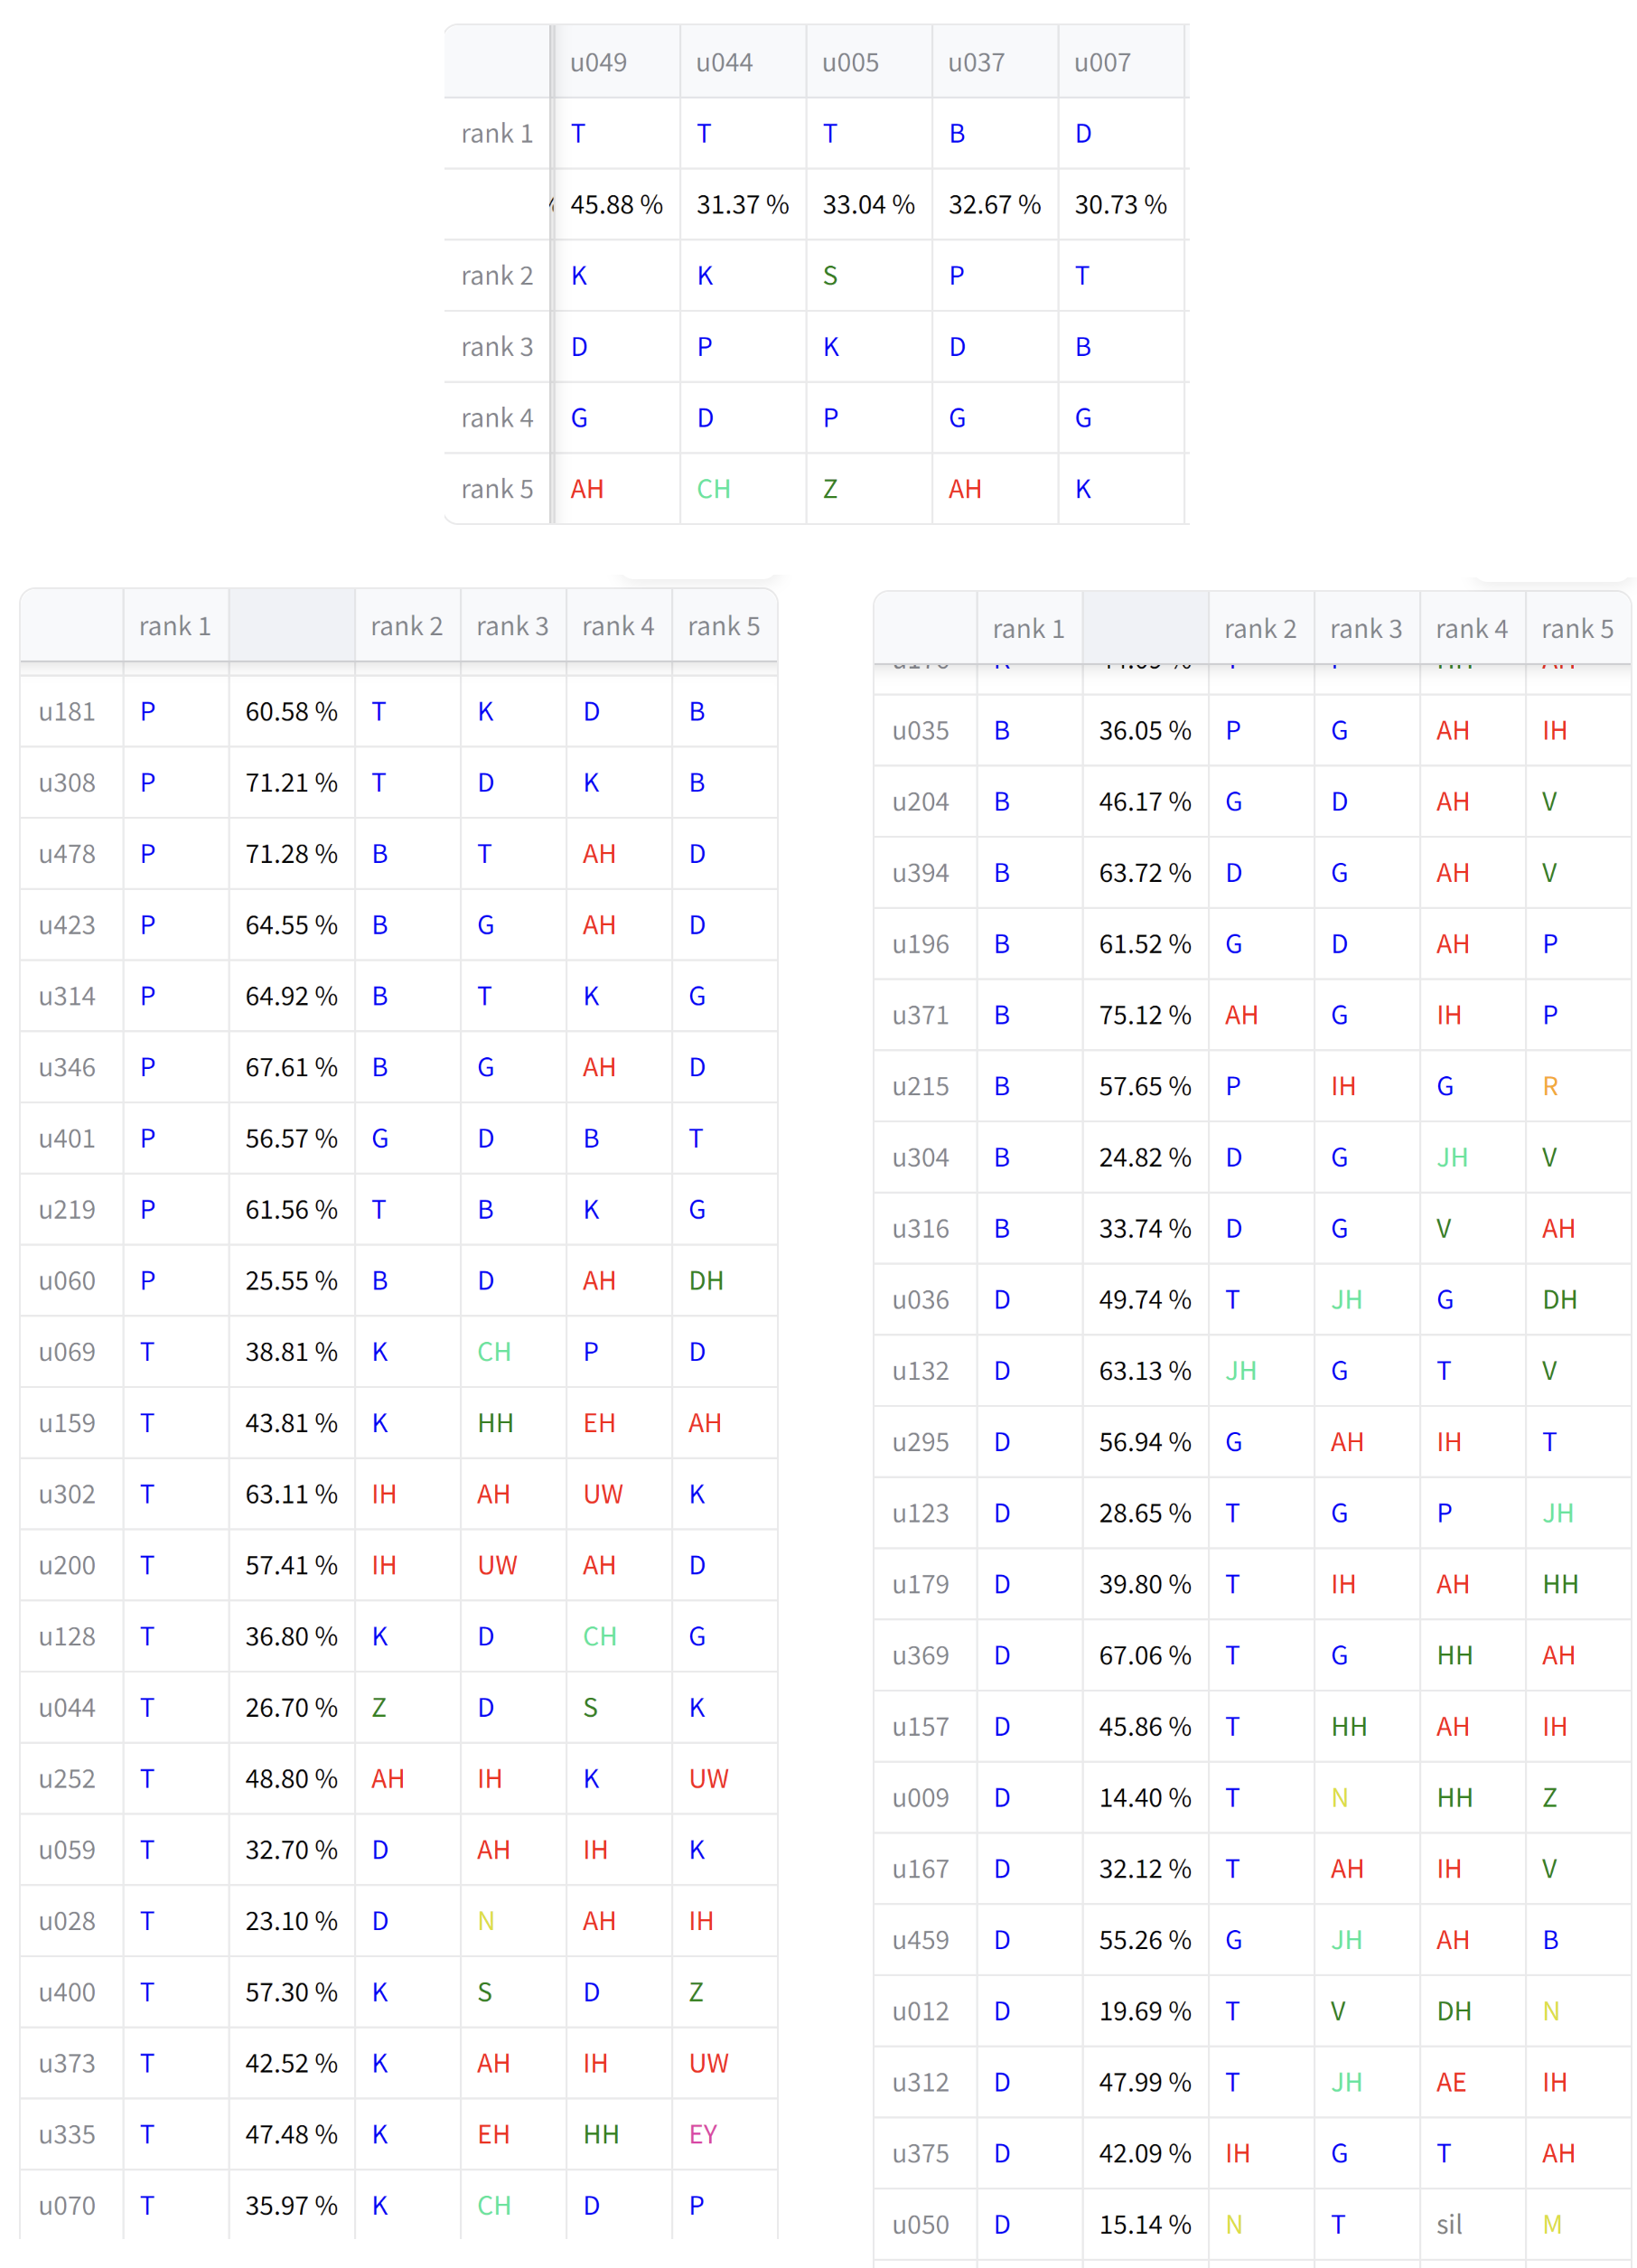
\includegraphics[width=\tempwidth]{figures/ch4figs/plo_phn.png}
                 \caption{塞音}
                 \label{fig:hub-u050-ap0500-ploobs}
             \end{subfigure}
             % \vfill
             % \begin{subfigure}{\textwidth}
             %     \centering
             %     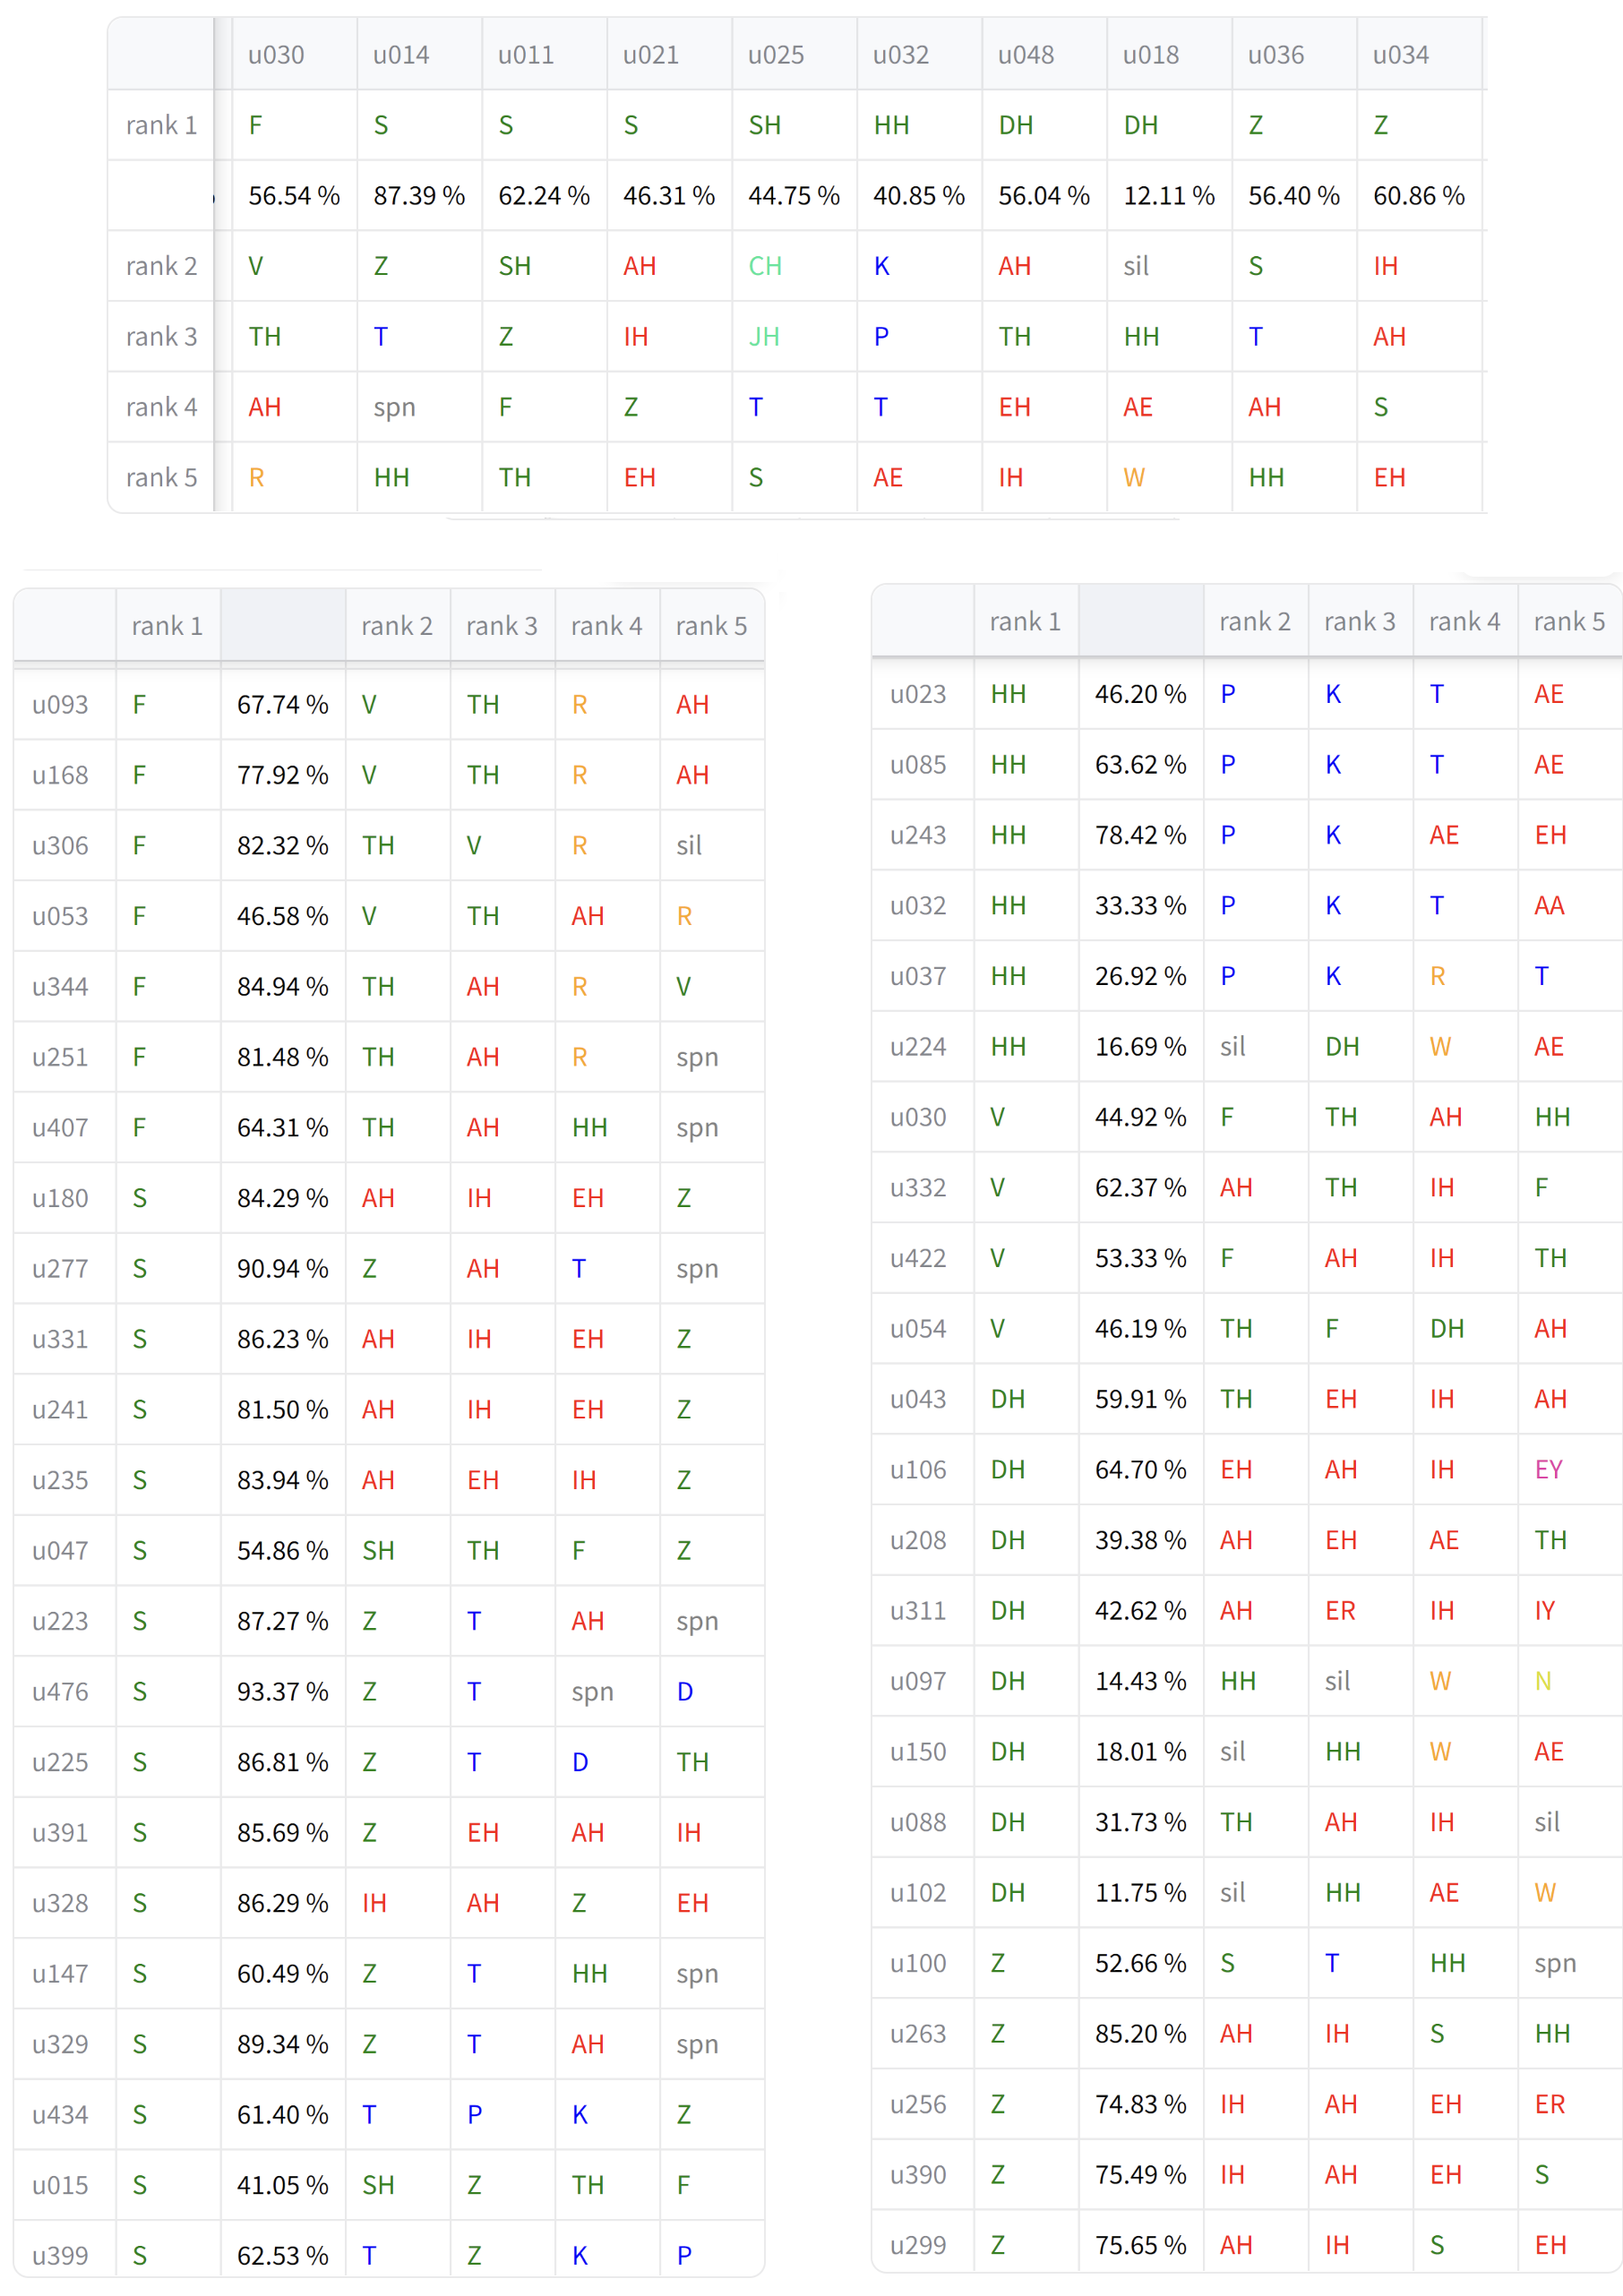
\includegraphics[width=\tempwidth]{figures/ch4figs/fri_phn.png}
             %     \caption{擦音}
             %     \label{fig:hub-u050-ap0500-friobs}
             % \end{subfigure}
             % \vfill
             % \begin{subfigure}{\textwidth}
             %     \centering
             %     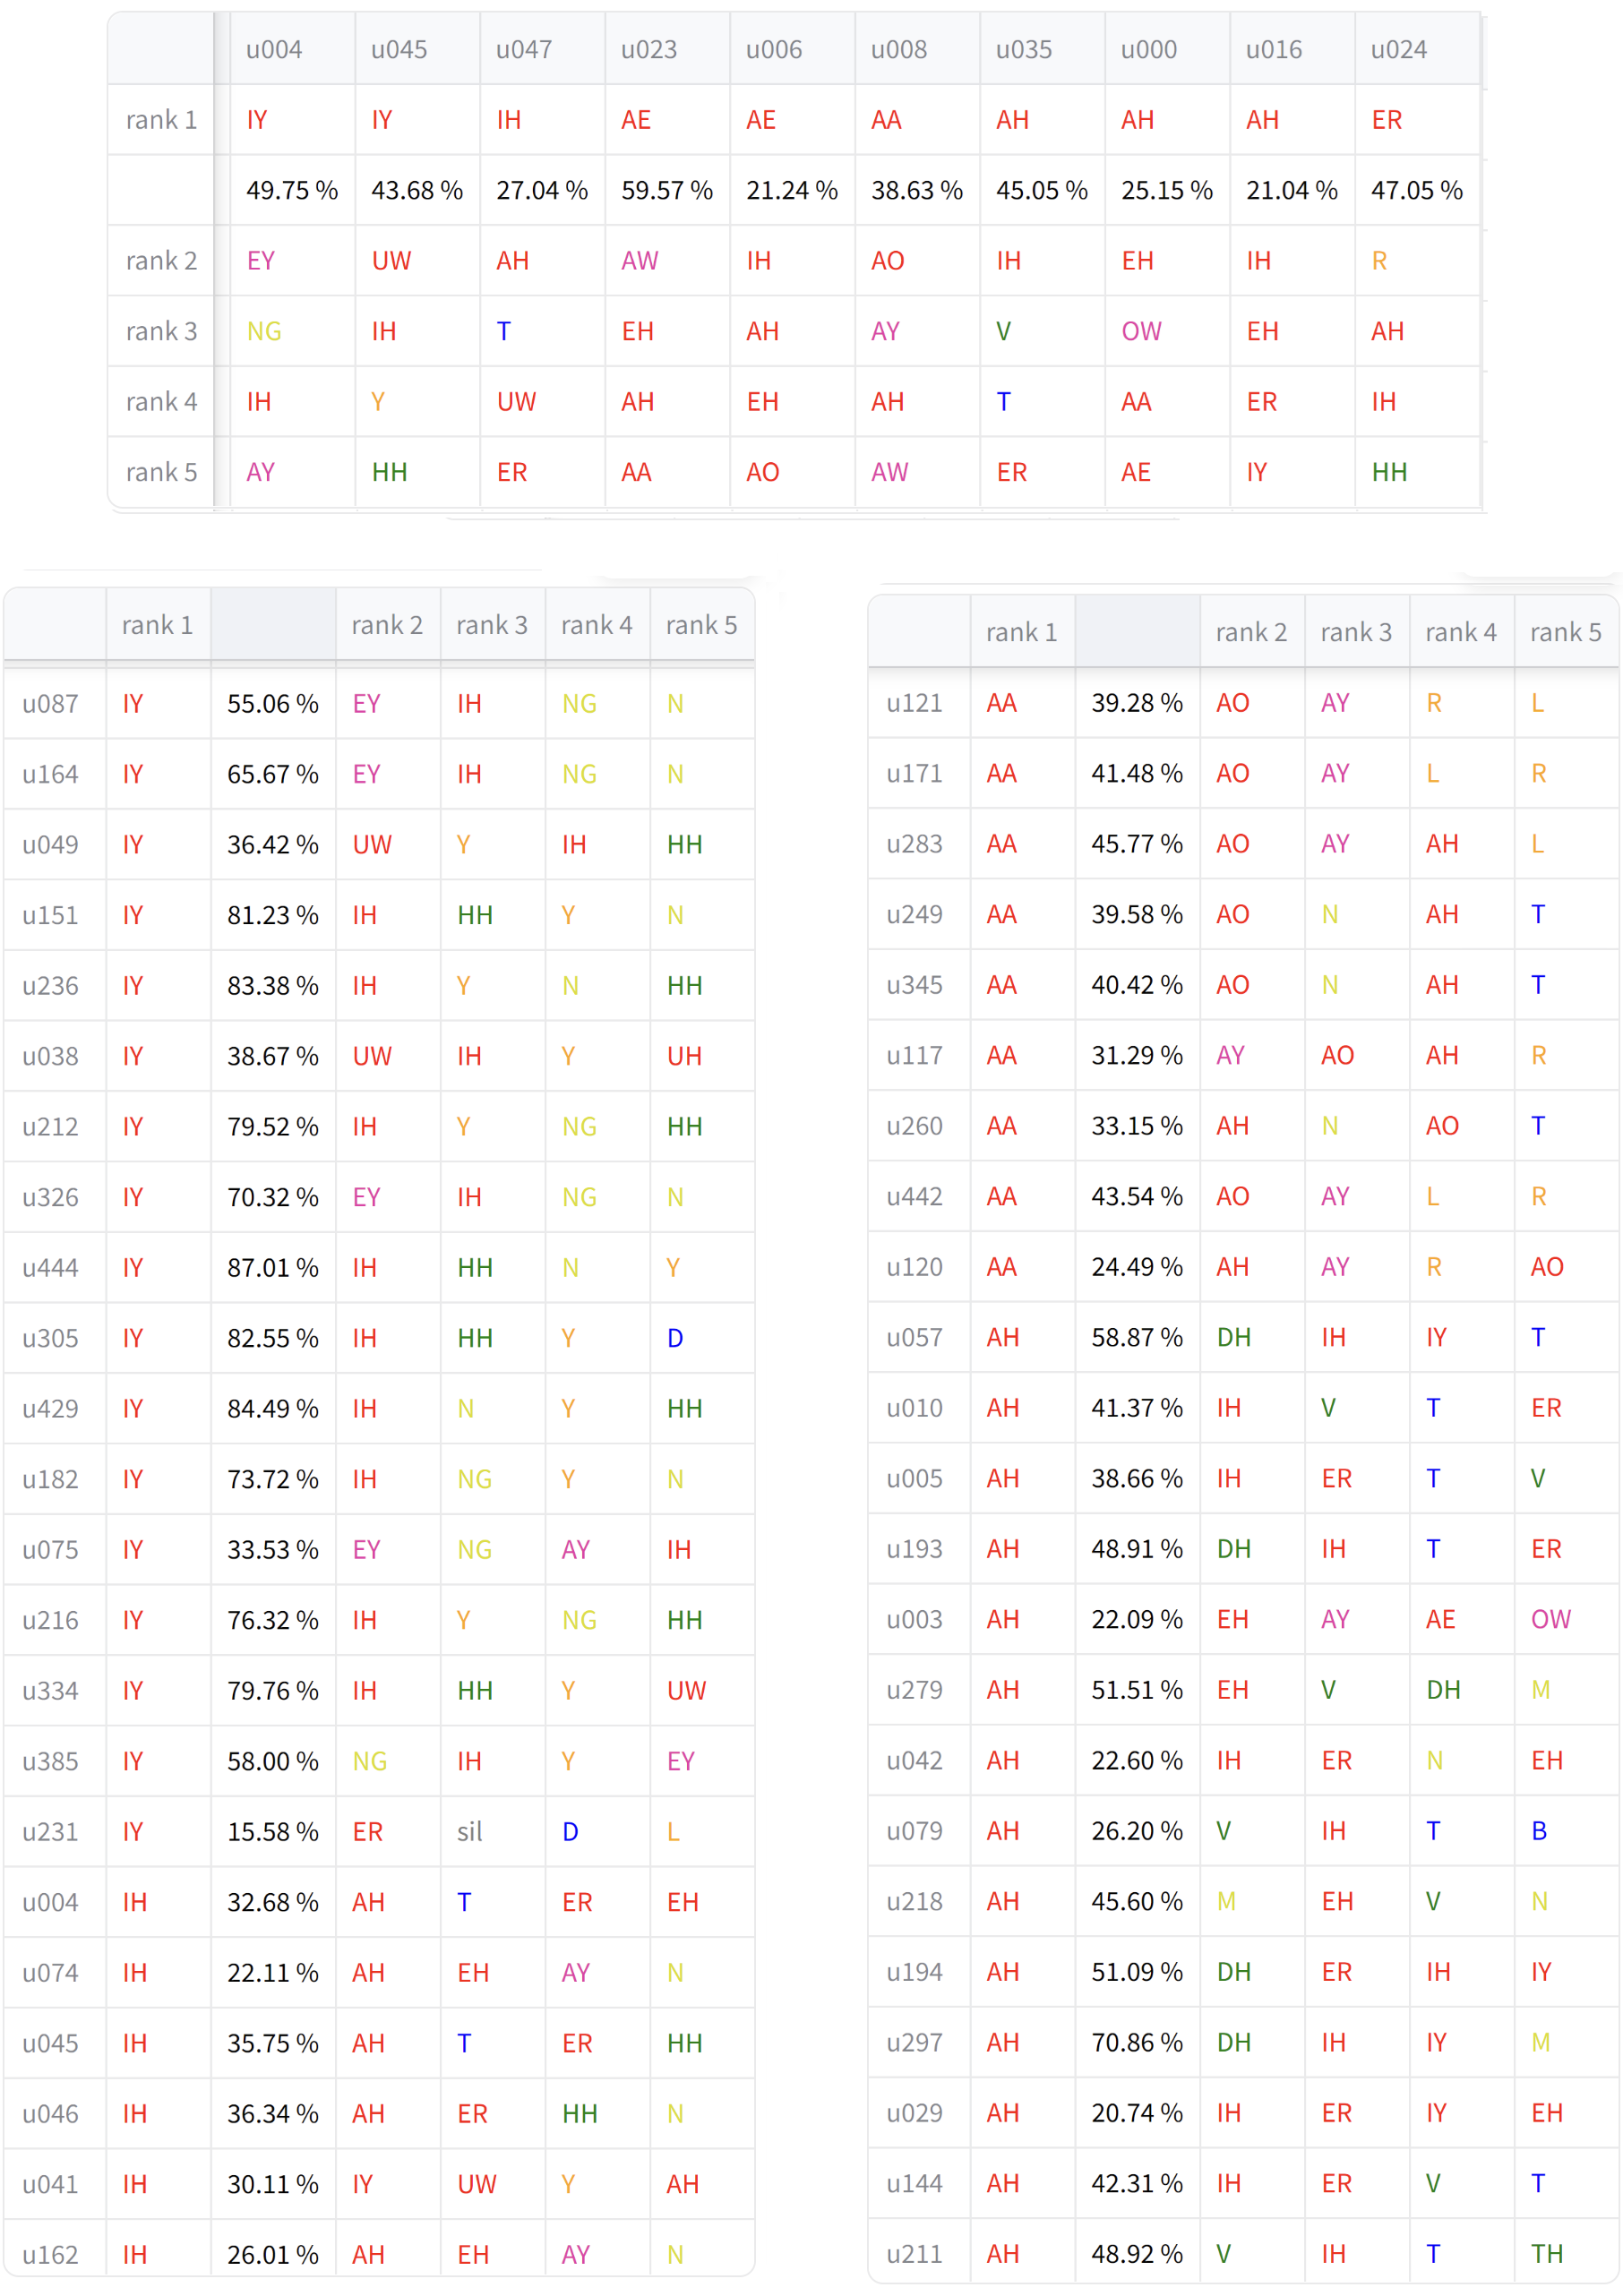
\includegraphics[width=\tempwidth]{figures/ch4figs/vow_phn.png}
             %     \caption{單元音}
             %     \label{fig:hub-u050-ap0500-vowobs}
             % \end{subfigure}

             \caption{HuBERT 表徵、K-平均演算法分群數 50,比較單一離散單元與}
             使用 500 種次詞單位,依據不同音位分類比較符記各自對應的前五高音位 \\
             上半部為離散單元,下半部為聲學片段。 \\
             圖中的百分比為最高機率音位的條件機率 $p_{y|z}(i^*(j)|j)$
                         \label{fig:hub-u050-phnobserver}
        \end{figure}
    }

        {
        \newcommand{\tempwidth}[0]{0.8\linewidth}
        \begin{figure}
        \ContinuedFloat
             \centering
             % \begin{subfigure}{\textwidth}
             %     \centering
             %     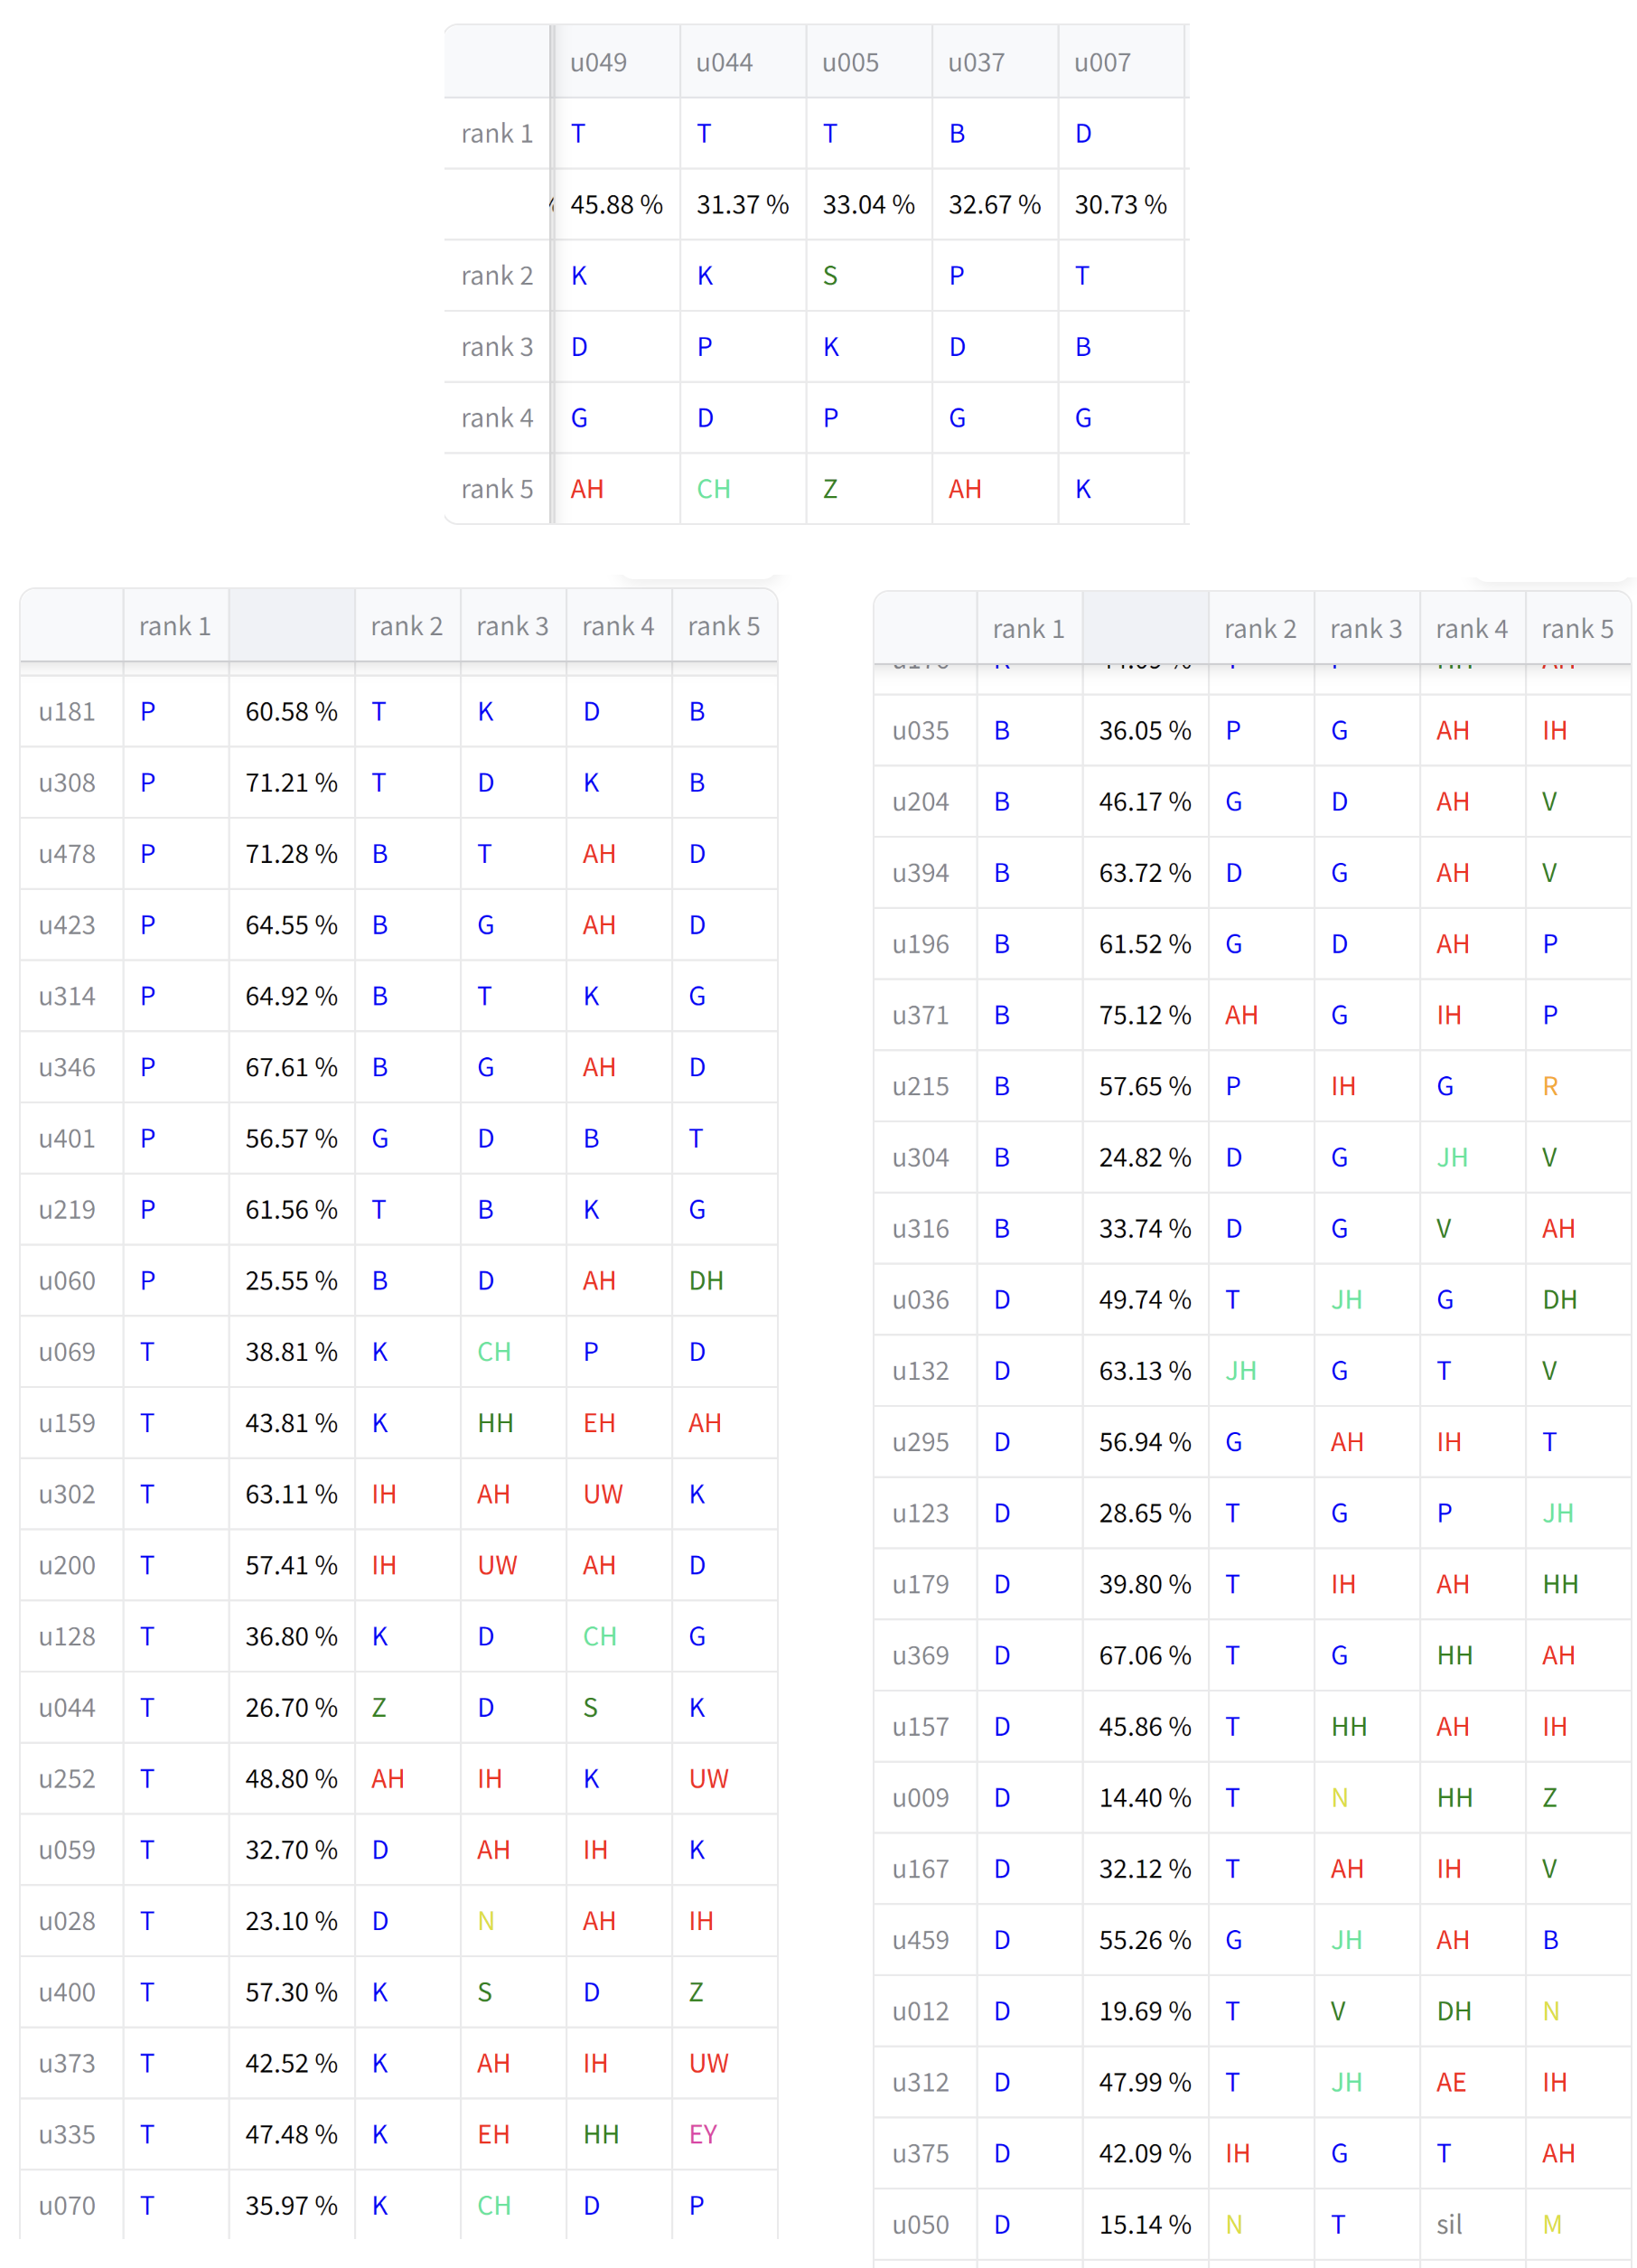
\includegraphics[width=\tempwidth]{figures/ch4figs/plo_phn.png}
             %     \caption{塞音}
             %     \label{fig:hub-u050-ap0500-ploobs}
             % \end{subfigure}
             % \vfill
             \begin{subfigure}{\textwidth}
                 \centering
                 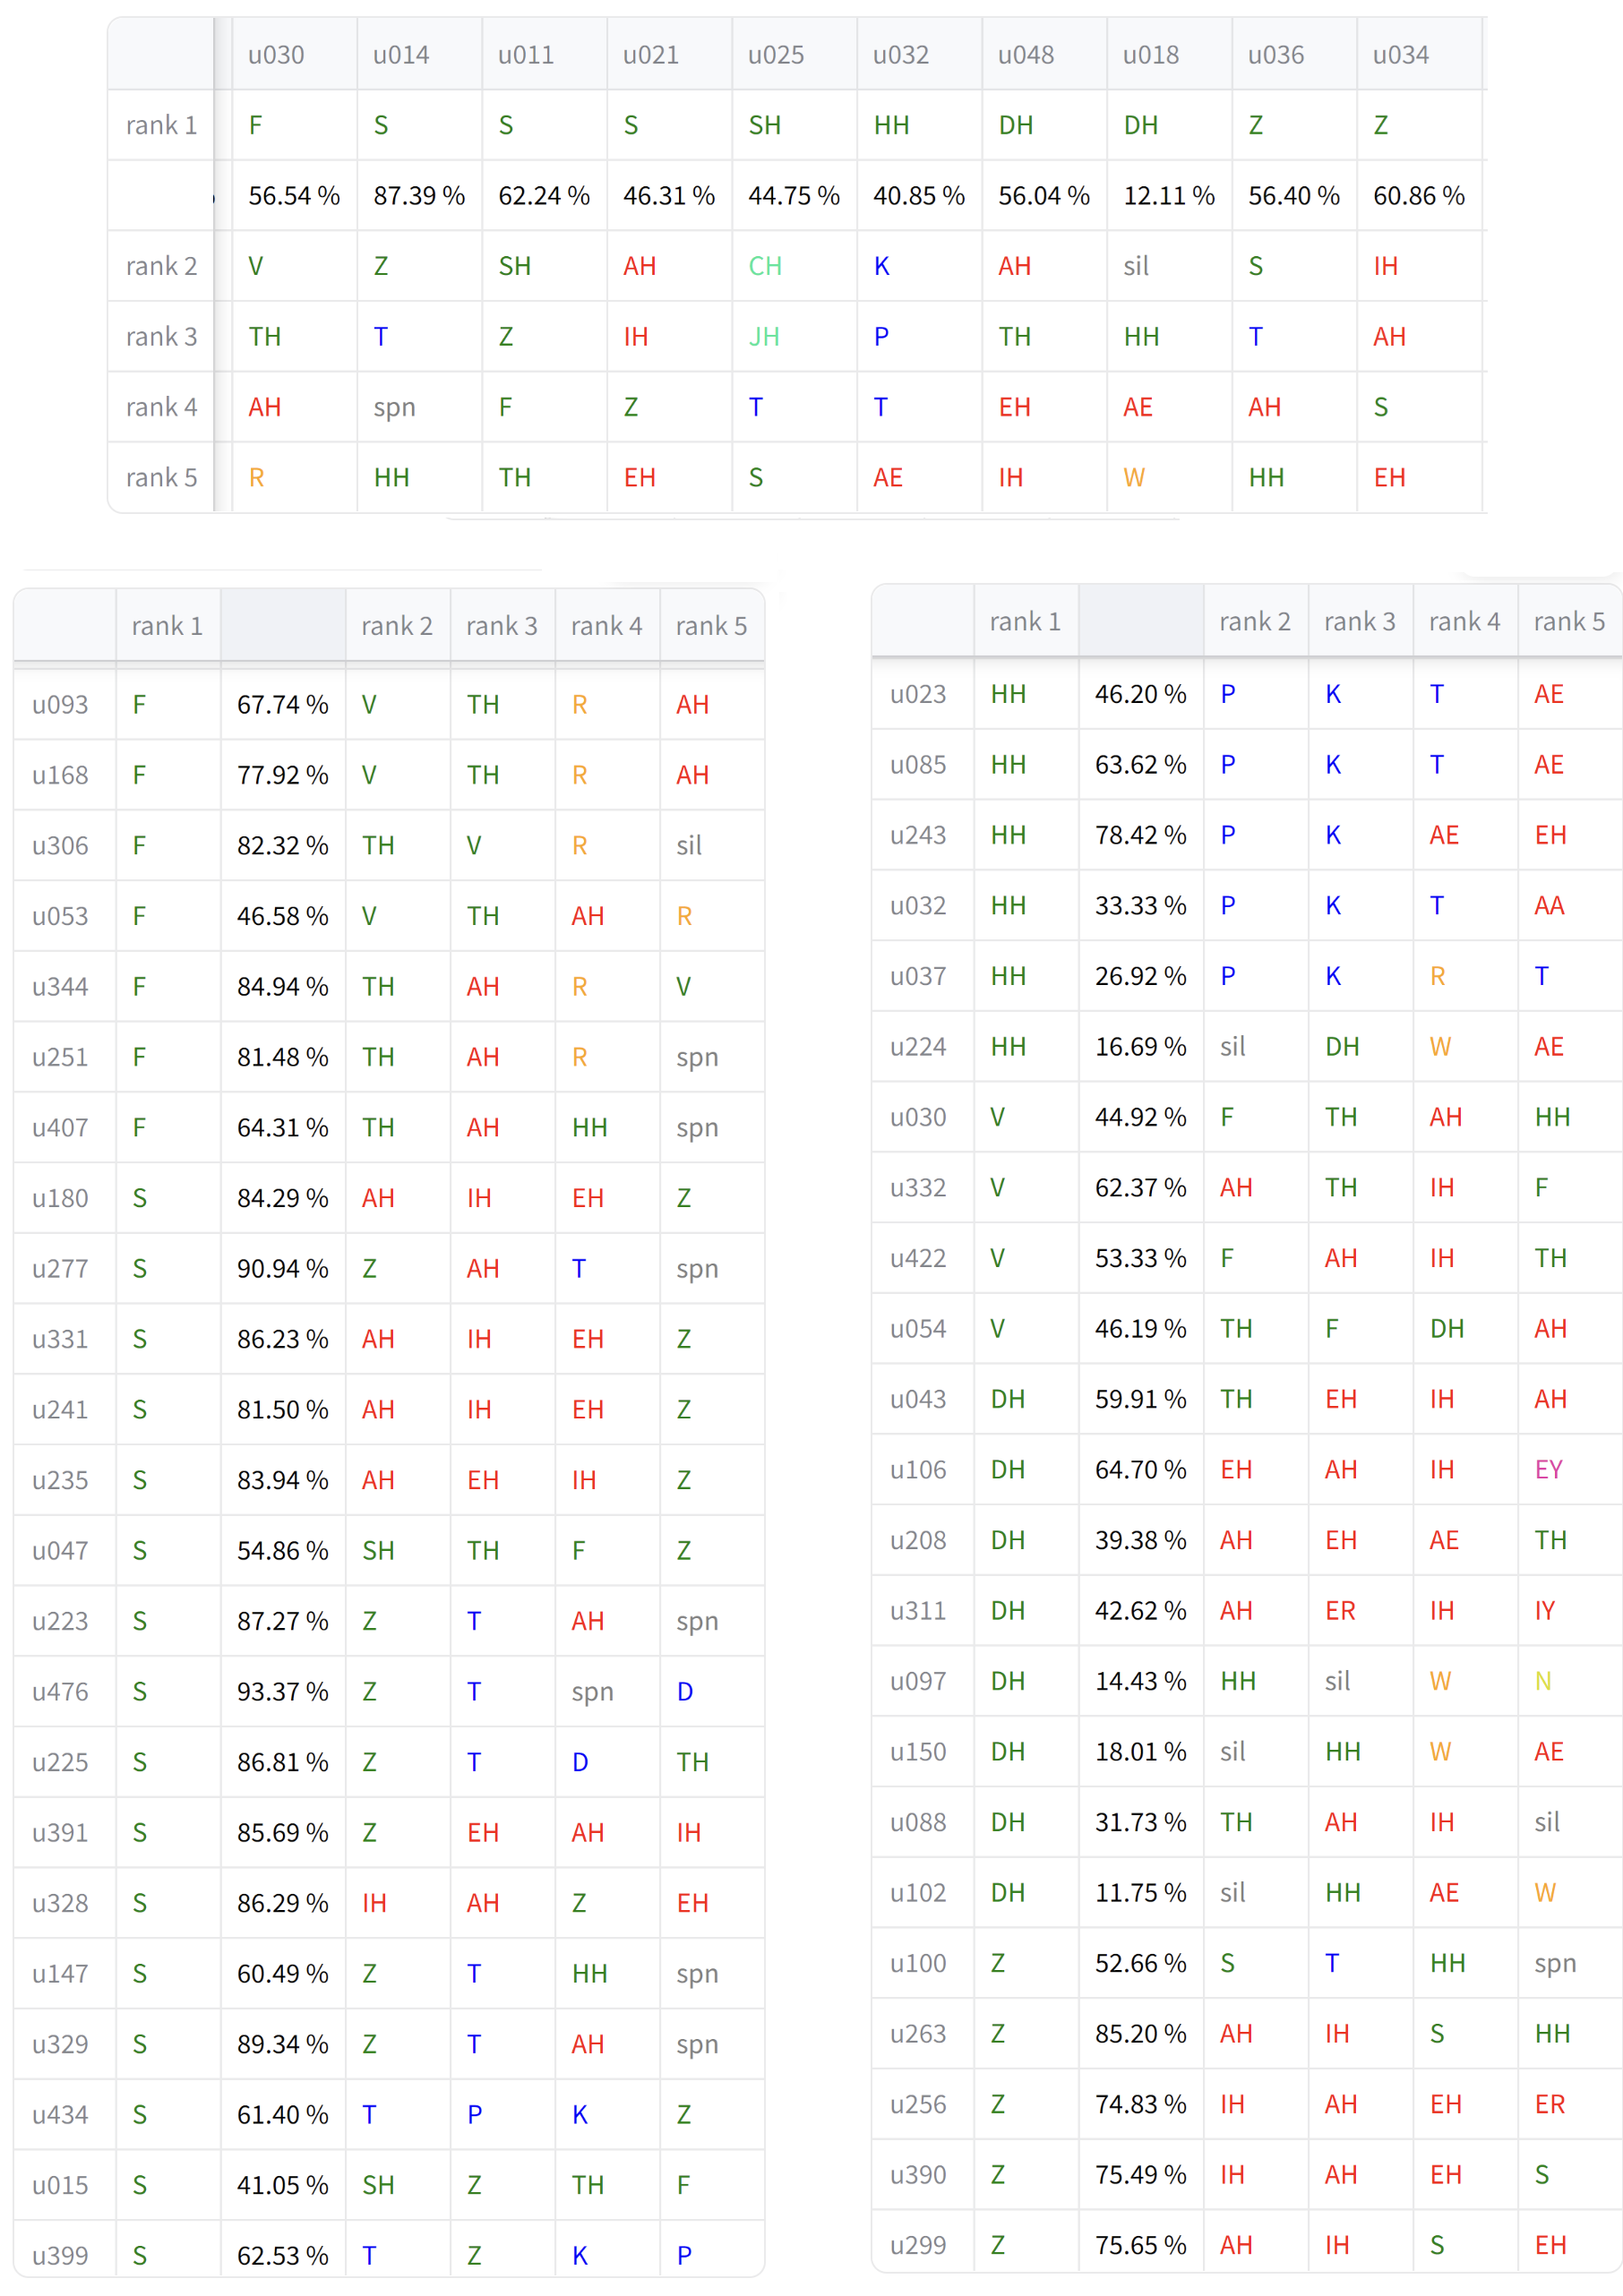
\includegraphics[width=\tempwidth]{figures/ch4figs/fri_phn.png}
                 \caption{擦音}
                 \label{fig:hub-u050-ap0500-friobs}
             \end{subfigure}
             % \vfill
             % \begin{subfigure}{\textwidth}
             %     \centering
             %     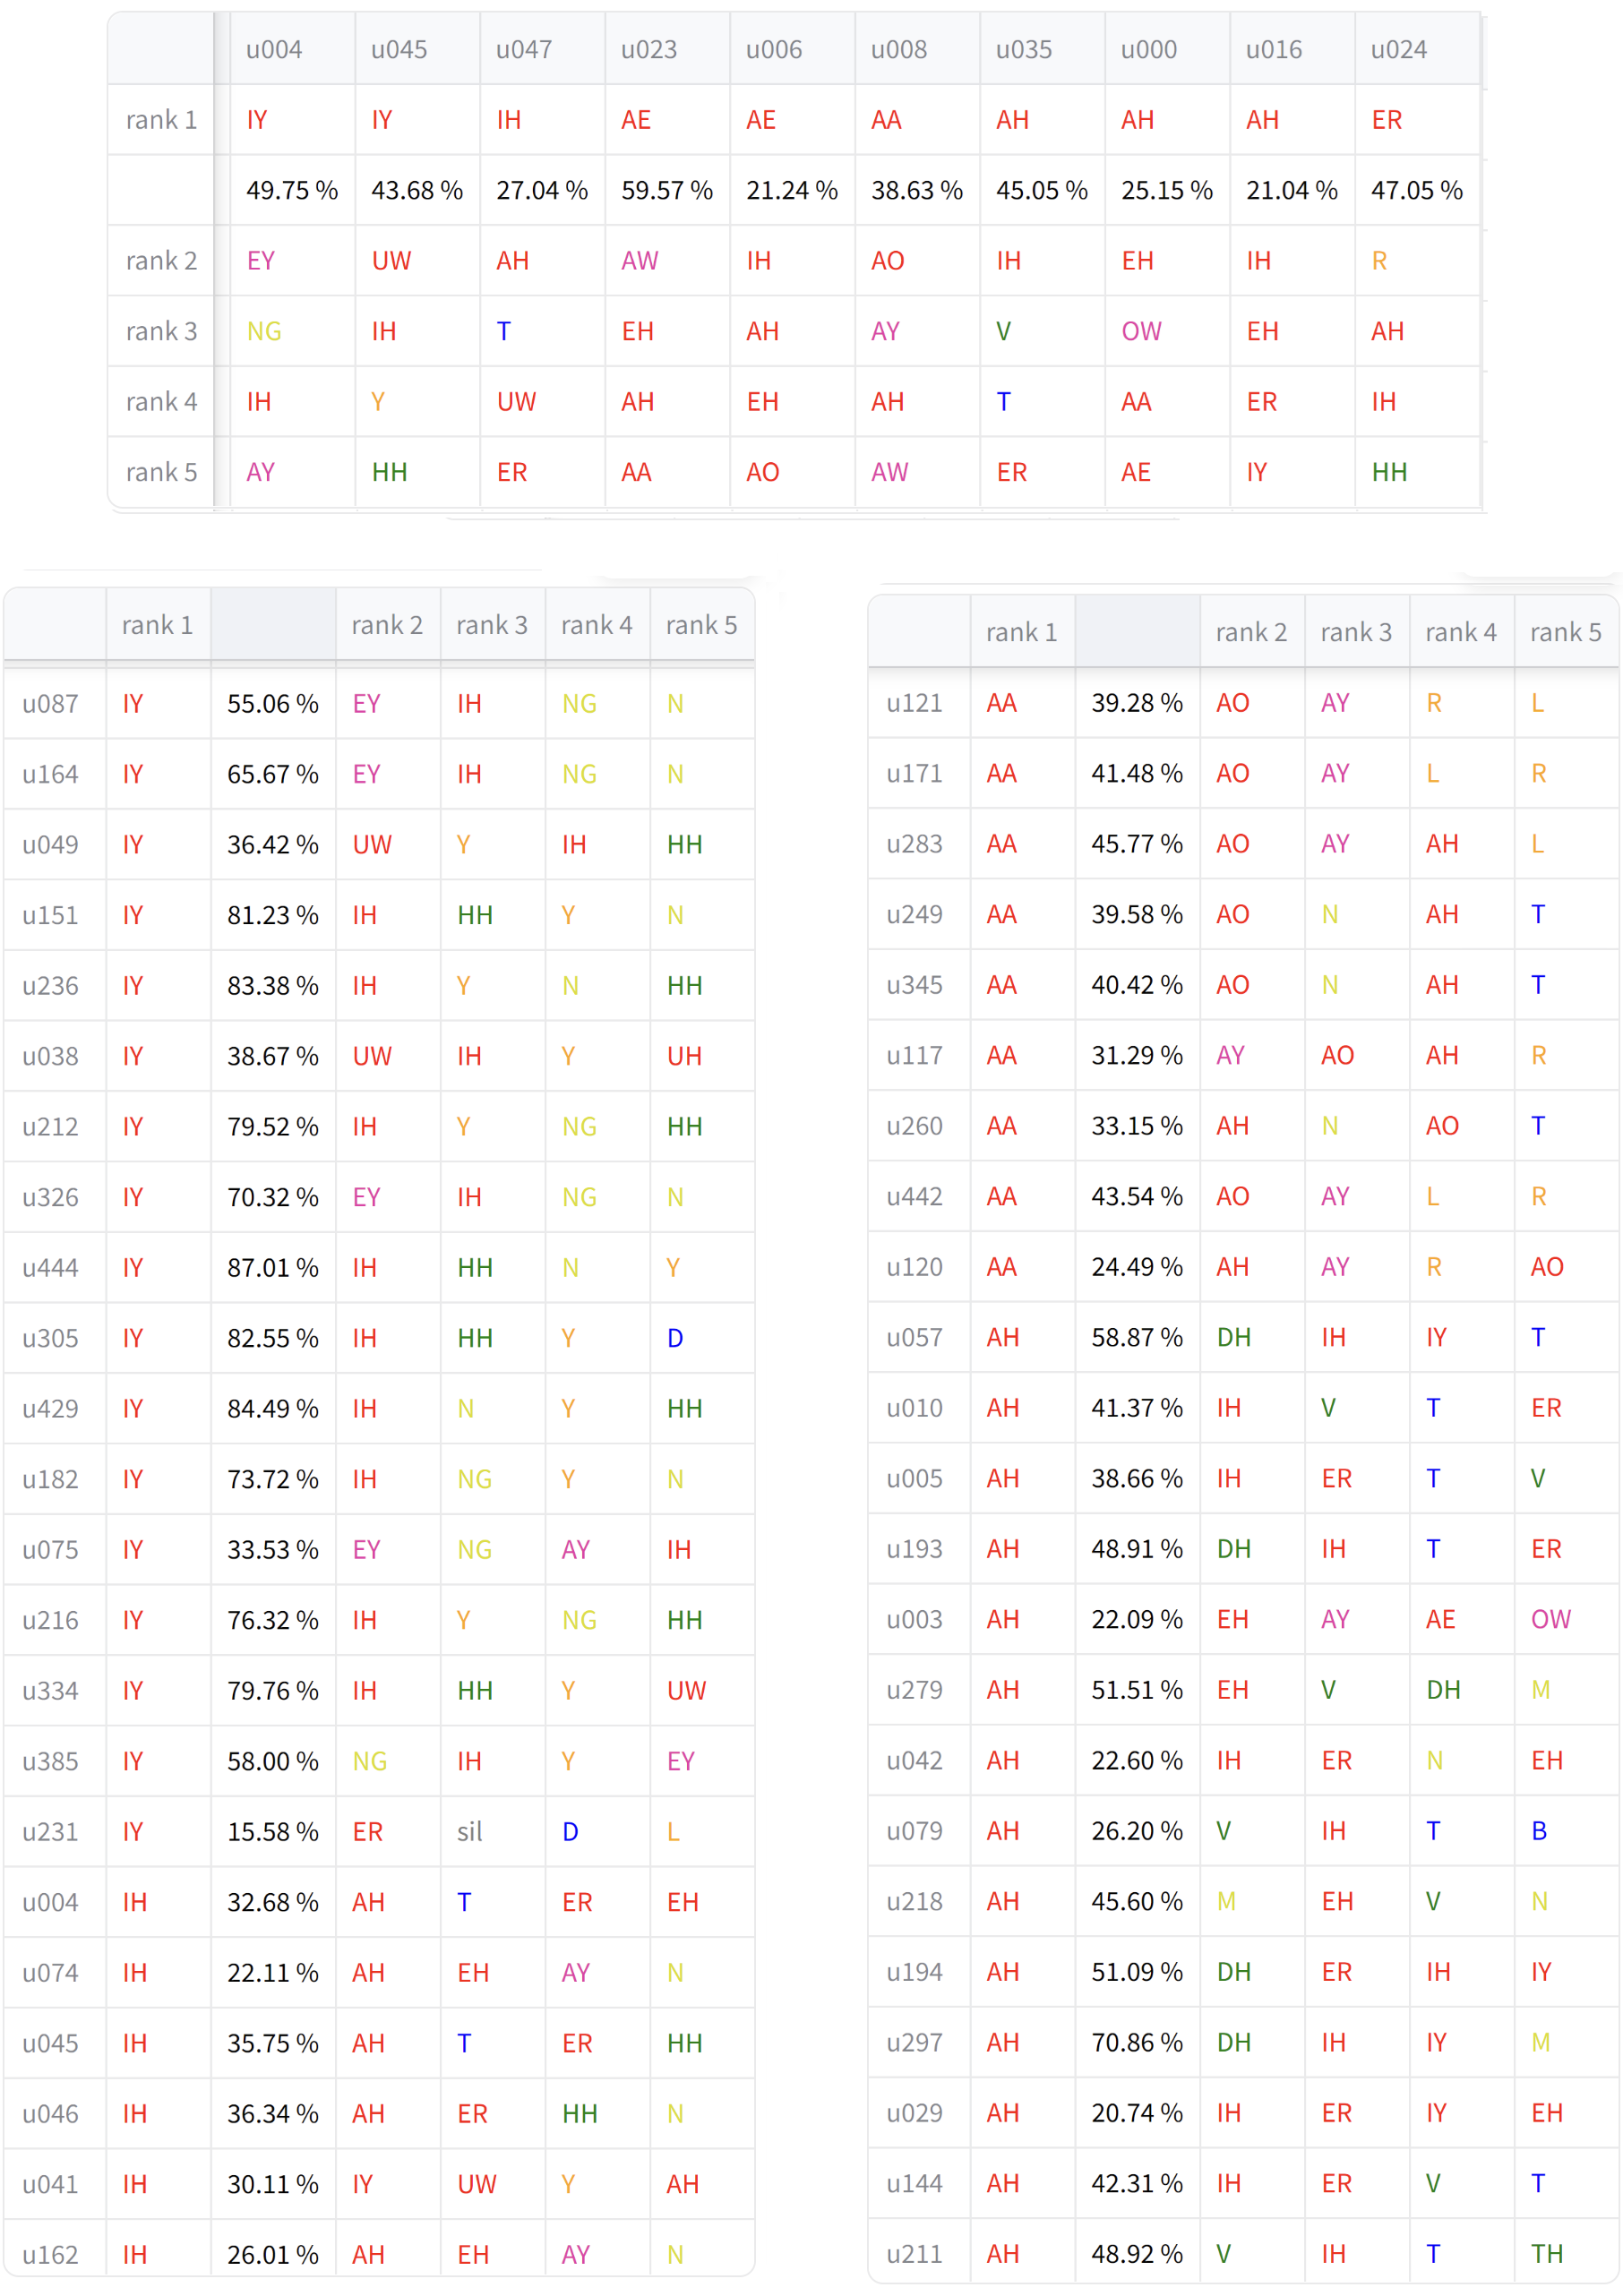
\includegraphics[width=\tempwidth]{figures/ch4figs/vow_phn.png}
             %     \caption{單元音}
             %     \label{fig:hub-u050-ap0500-vowobs}
             % \end{subfigure}

             % \caption{HuBERT 表徵、K-平均演算法分群數 50,比較單一離散單元與使用 500 種次詞單位,}
             % 依據不同音位分類比較符記各自對應的前五高音位
             % (上半部為離散單元,下半部為聲學片段。圖中的百分比為最高機率音位的條件機率 $p_{y|z}(i^*(j)|j)$)
                         \label{fig:hub-u050-phnobserver--2}
        \end{figure}
    }

        {
        \newcommand{\tempwidth}[0]{0.8\linewidth}
        \begin{figure}
        \ContinuedFloat
        
             \centering
             % \begin{subfigure}{\textwidth}
             %     \centering
             %     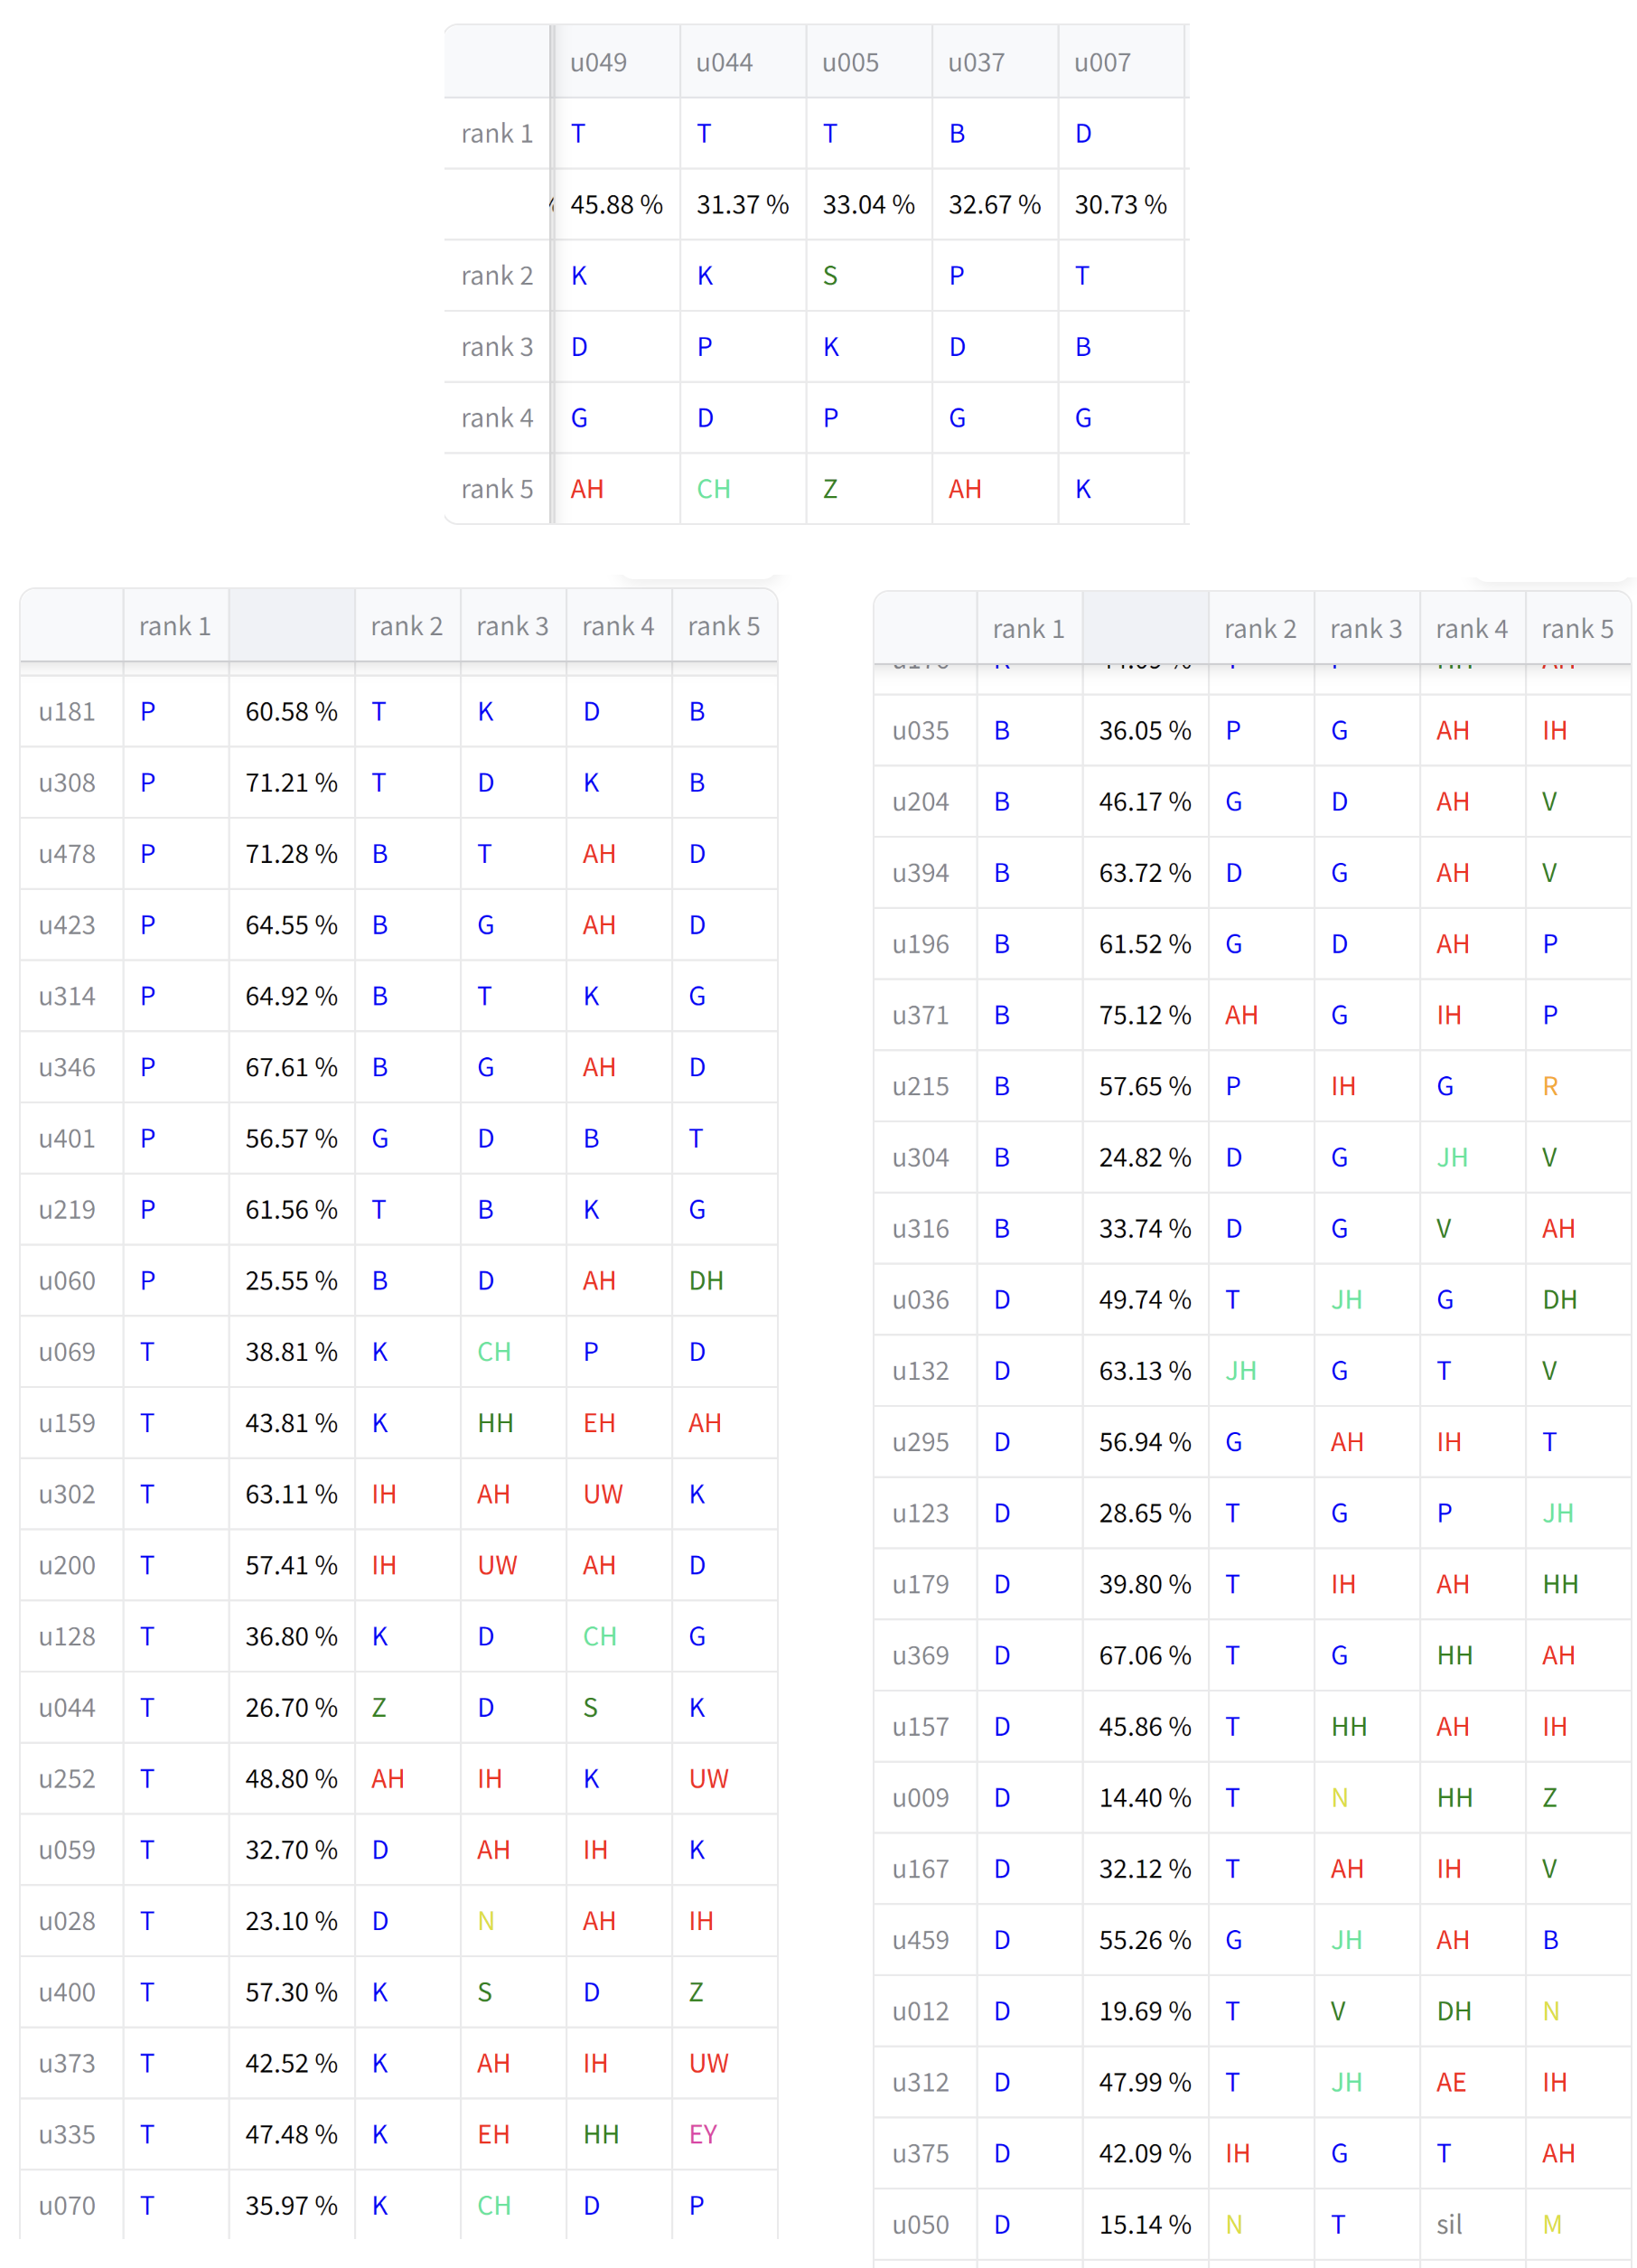
\includegraphics[width=\tempwidth]{figures/ch4figs/plo_phn.png}
             %     \caption{塞音}
             %     \label{fig:hub-u050-ap0500-ploobs}
             % \end{subfigure}
             % \vfill
             % \begin{subfigure}{\textwidth}
             %     \centering
             %     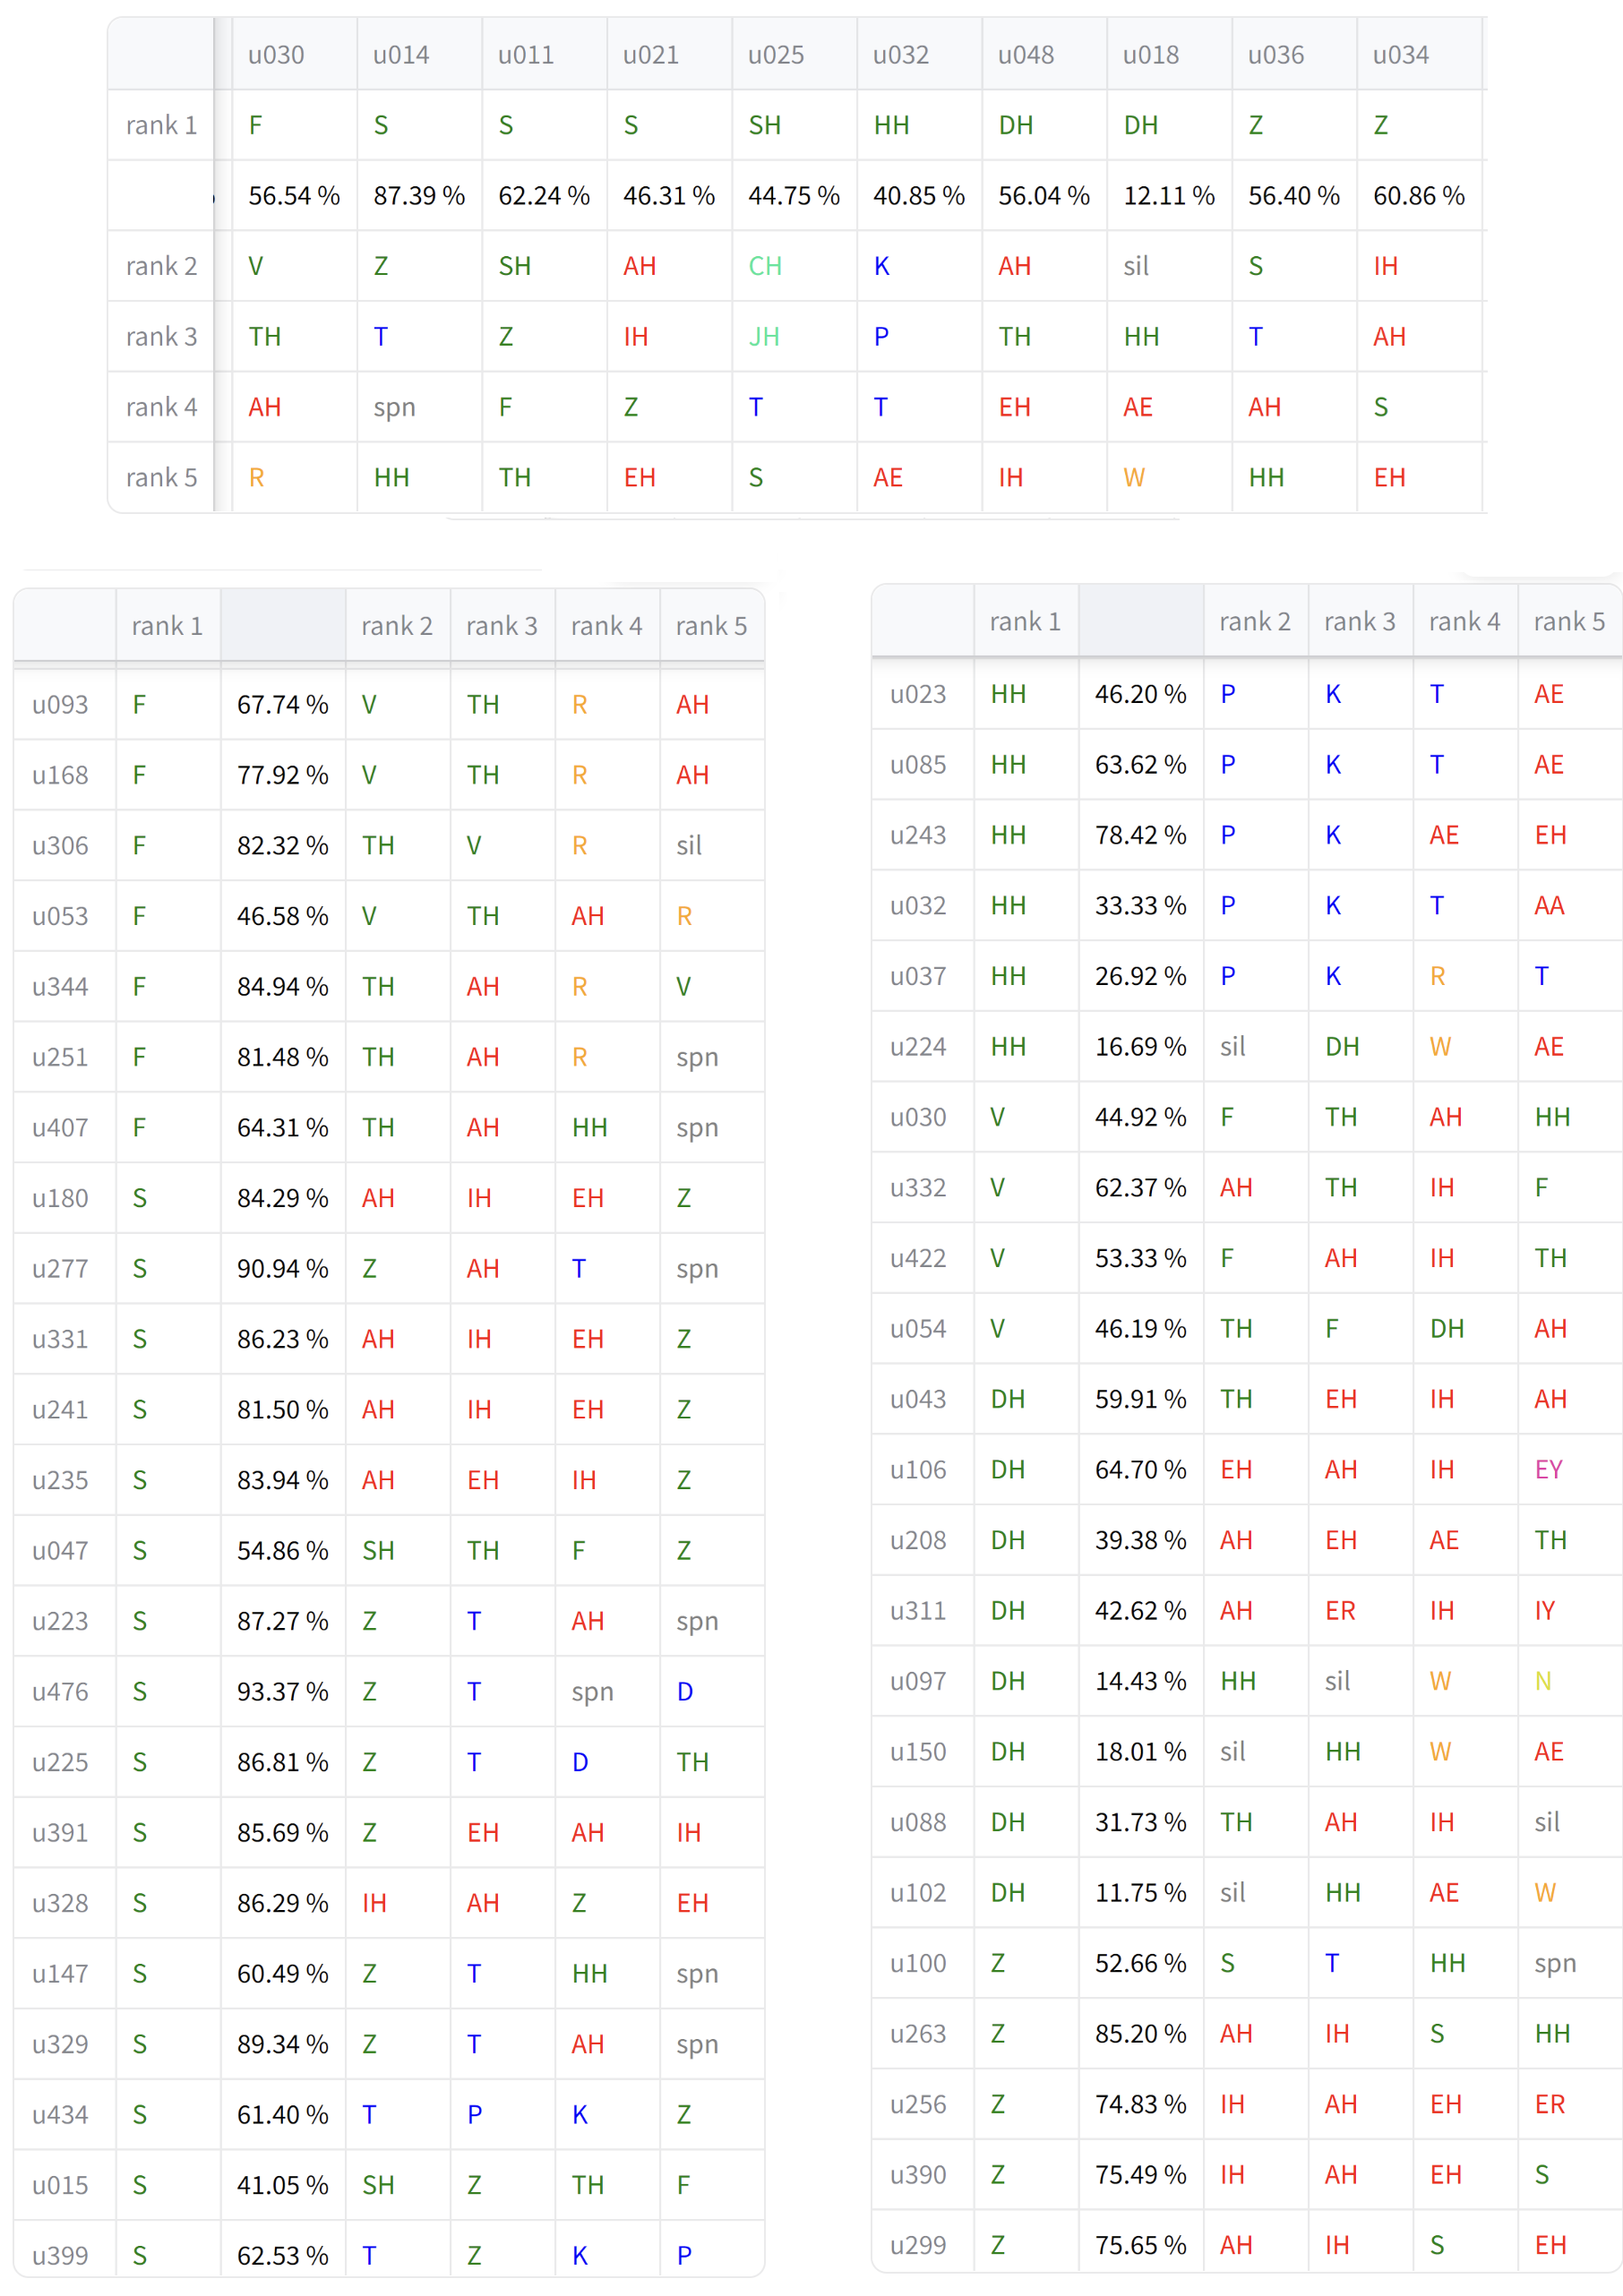
\includegraphics[width=\tempwidth]{figures/ch4figs/fri_phn.png}
             %     \caption{擦音}
             %     \label{fig:hub-u050-ap0500-friobs}
             % \end{subfigure}
             % \vfill
             \begin{subfigure}{\textwidth}
                 \centering
                 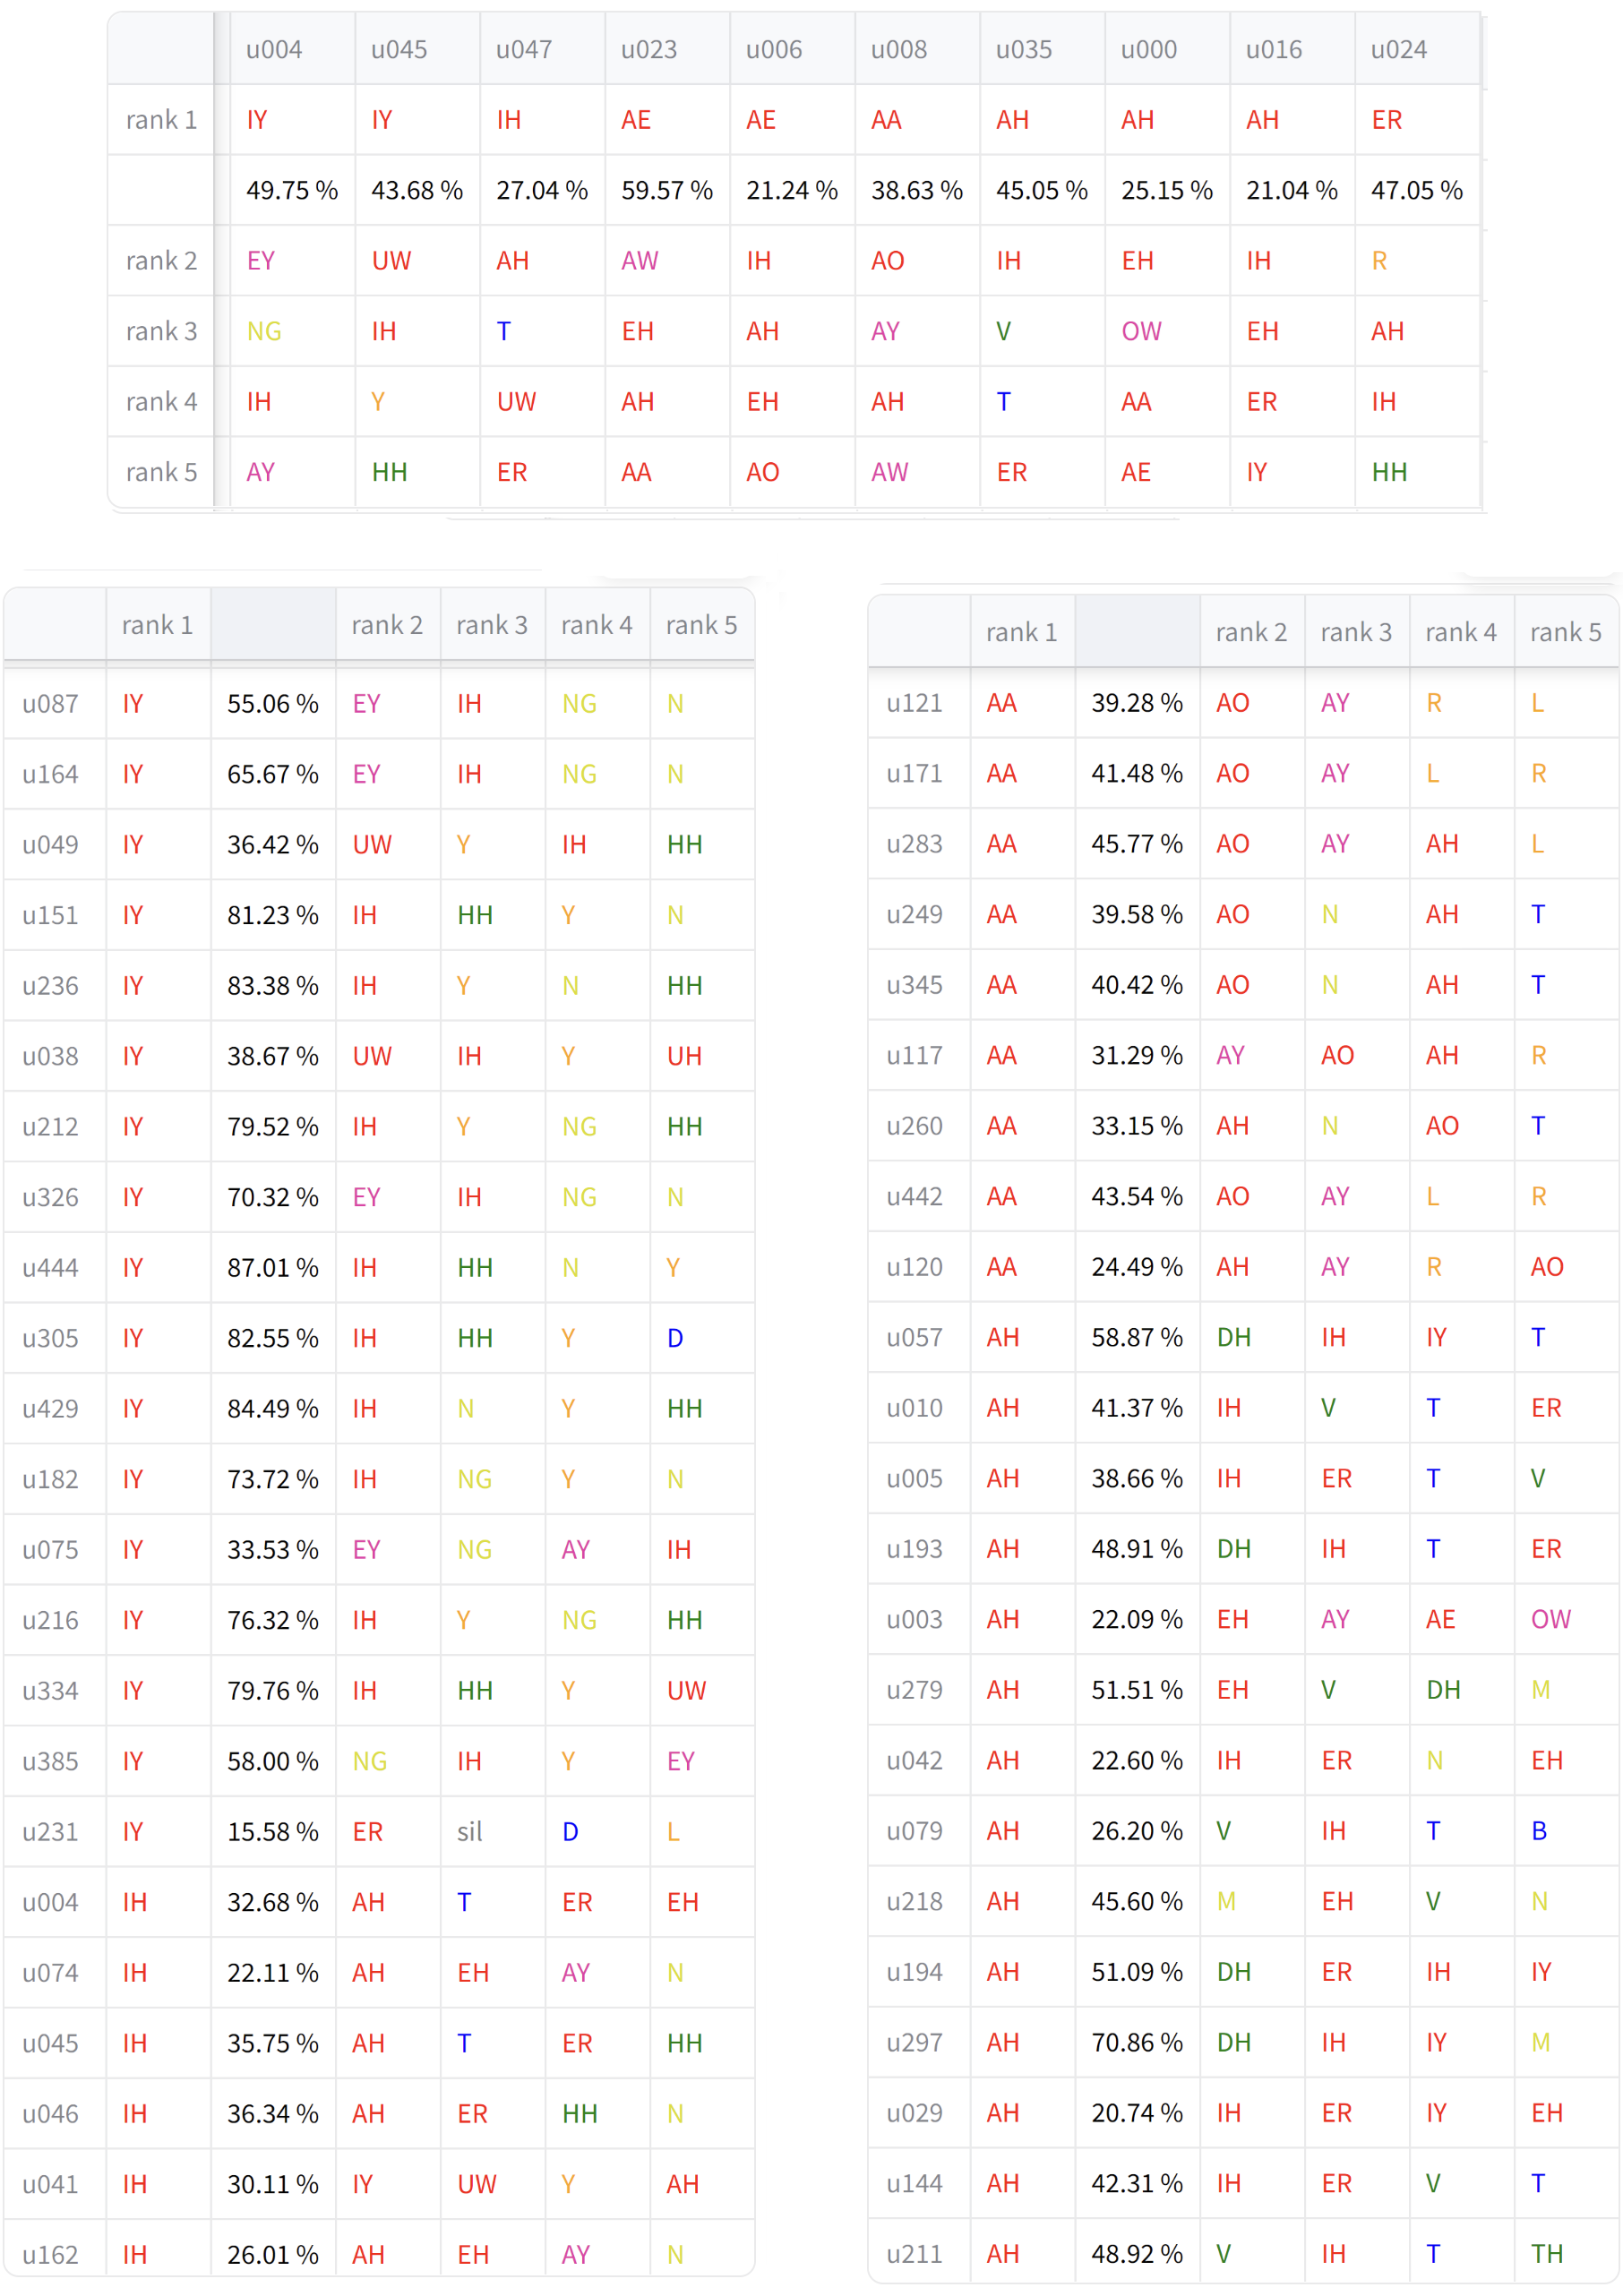
\includegraphics[width=\tempwidth]{figures/ch4figs/vow_phn.png}
                 \caption{單元音}
                 \label{fig:hub-u050-ap0500-vowobs}
             \end{subfigure}

             % \caption{HuBERT 表徵、K-平均演算法分群數 50,比較單一離散單元與使用 500 種次詞單位,}
             % 依據不同音位分類比較符記各自對應的前五高音位
             % (上半部為離散單元,下半部為聲學片段。圖中的百分比為最高機率音位的條件機率 $p_{y|z}(i^*(j)|j)$)
                         \label{fig:hub-u050-phnobserver--3}
        \end{figure}
    }
